\section{The Pluvian Forest}

\subsubsection{About the Region}

The Pluvian Forest is the name of the forest that is located to the North of Aurushire. The forest is known for strange spacial occurrences happening within it. Those who travel into The Pluvian Forest do not generally return or will return very confused or changed.

\subsubsection{Unique Forest Dynamics}

The Pluvian Forest is largely effected by the contents of the Spati Aethereu Thalamun (Aethereu). It is a normal forest in itself but it's close proximity to Aethereu makes this region dangerous. The forest is heavily affected by the space stone such that visitors can be lost for weeks while only traveling through a few days worth of terrain. Similarly, the time stone has the strongest connection to the space stone and thus has a great influence on the area. Often, travelers find the days lasting longer or shorter than usual. The energy stone has an effect on this region which amplifies the effect of the other two stones.

\begin{commentbox}{Irregular Days}
	As a byproduct of the time stone effecting the region, often the days find themselves to be shortened or lengthened due to the time stone effect from Aethereu. As a DM, you can determine periodically if there is any effect on travelers by rolling a 1d20 and succeeding a DC11 time throw. If failed, roll a 1d20 to determine the effect on the party.
	\hline
	\begin{description}
		\item[1:] Party transported 1 year into the future. 
		\item[2:] Party transported 3 months into the future. This may induce a season change. 
		\item[3:] Party transported 2 weeks into the future. This may induce a temperature change.
		\item[4-5:] Party transported 1 day into the future. 
		\item[6-7:] Party transported 5 hours into the future. 
		\item[8-10:] Party transported 1 hour into the future. 
		\item[11-13:] Party transported 1 hour into the past. 
		\item[14-15:] Party transported 5 hours into the past. 
		\item[16-17:] Party transported 1 day into the past. 
		\item[18:] Party transported 2 weeks into the past. This may induce a temperature change. 
		\item[19:] Party transported 3 months into the past. This may induce a season change. 
		\item[20:] Party transported 1 year into the past. 
	\end{description}
\end{commentbox}

\begin{commentbox}{Irregular Creatures}
	As a byproduct of the time stone working in conjunction with the space stone effecting the region, often creatures of objects of strange origin can appear in the area. As a DM, you can determine periodically if there is any effect on travelers by rolling a 1d20 and succeeding a DC13 space-time throw. If failed, roll a 1d20 to determine the effect on the party.
	\hline
	\begin{description}
		\item[1:] A prehistoric dinosaur appears in a nearby area.
		\item[2:] A long known-to-be extinct creature appears in a nearby area.
		\item[3:] A creature not native to this area appears in a nearby area.
		\item[4:] An ancient item appears in a nearby area.
		\item[5-6:] A creature native to the area appears behind the party.
		\item[7-10:] An item owned by a player vanishes and teleports to a location shortly behind them on their path.
		\item[11-14:] An item owned by a player vanishes and teleports to a location shortly ahead of them on their path.
		\item[15-16:] A creature native to the area appears ahead of the party.
		\item[17:] A futuristic item appears in a nearby area.
		\item[18:] A creature not native to this area appears in the nearby area.
		\item[19:] A natural creature that has never been seen before appears in the area.
		\item[20:] A robotic creature appears in the area.
	\end{description}
\end{commentbox}

\begin{commentbox}{Irregular Movement}
	As a byproduct of the space stone effecting the region, often the part finds themselves being moved around to different areas or places they have been before. As a DM, you can determine periodically if there is any effect on travelers by rolling a 1d20 and succeeding a DC15 space throw. If failed, roll a 1d20 to determine the effect on the party.
	\hline
	\begin{description}
		\item[1:] One member of the party is teleported to the entrance of The Pluvian Forest.
		\item[2:] The party members are teleported to a random location in The Pluvian Forest (chosen by the DM or completely random).
		\item[3:] The party is instantly moved to the last place they teleported from. If they have not been teleported yet, nothing will happen.
		\item[4:] Roll a DC12 save. Upon failing, the party is teleported to Rem Silvia.
		\item[5-6:] An object being carried by a member of the party is teleported just behind them on their path.
		\item[7-8:] The party is turned around.
		\item[9- 10:] The party is teleported to a place just ahead of where they weree. If they pass a DC15 perception check they will know they have moved. 
		\item[11-12:] The party is teleported to a place they recently were. If they pass a DC15 perception check they will know they have moved. The party may see tracks left by them which would lead them back to where they were.
		\item[13-14:] The party is turned around.
		\item[15-16:] An object being carried by a member of the party is teleported just ahead of them on their path. 
		\item[17:] Roll a DC12 save. Upon failing, the party is teleported to Aurushire.
		\item[18:] The party is instantly moved to the last place they teleported from. If they have not been teleported yet, nothing will happen.
		\item[19:] The party members are teleported to a random location in The Pluvian Forest (chosen by the DM or completely random).
		\item[20:] One member of the party is teleported to the end of The Pluvian Forest.
	\end{description}
\end{commentbox}

\begin{commentbox}{Irregular Energy}
	As a byproduct of the energy stone effecting the region, often creatures are either not as strong as they seem or have extraordinary strength. As a DM, you can determine periodically if there is any effect on travelers by rolling a 1d20 and succeeding a DC11 energy throw. If failed, roll a 1d20 to determine the effect on the party.
	\hline
	\begin{description}
		\item[1-5:] A member of the party acquires a level of exhaustion.
		\item[6:] A member of the party loses a spell slot.
		\item[7:] A member of the party loses 10 HP.
		\item[8-10:] A creature has all of its strength sapped and is very easy to defeat.
		\item[11-15:] Objects or areas of the forest glow and irradiate magical power. This can be trees, a stream, a pond, creatures, the ground, the path, or anything else. 
		\item[16-17:] A creature of the forest is bestowed with extraordinary strength (depending on party condition).
		\item[18:] A member of the party gains 10 HP. 
		\item[19:] A member of the party gains a missing spell slot. 
		\item[20:] A member of the party loses a level of exhaustion.
	\end{description}
\end{commentbox}

\subsubsection{Navigating The Pluvian Forest}

In order to successfully navigate through The Pluvian Forest and find Aethereu, the party must follow a simple set of instructions, while not getting turned around by the irregular occurrences. These set of instructions may be given to the party in a variety of ways (see below). 

\begin{commentbox}{Successful Navigation}
	\begin{description}
		\item[Guidence of Time] When nature calls, you must follow it's guidance. You must follow the hoot of the owls and the sounds of the wolves.
		\item[Guidence of Space] The correct path points to the stars. Follow the hills up and not down.
		\item[Guidence of Energy] The forest seeks to distract. Avoid illusions created by the energy stone.
		\item[Guidence of the Trinity] When the trinity is broken, search for the missing link. When two of the rules above are broken, look for the third to act.
	\end{description}
\end{commentbox}

\subsection{NPC's}

All of the creatures that can appear in The Pluvian forest are the same as those of Rem Silva Except the night elves and Rexxar/Bella. Similarly, the party can encounter a number of various other creatures.

\subsection{Encounters and Discoveries}

Throughout the forest, many things can happen to the party including visions/dreams, strange occurrences, interesting discoveries, and more.

\begin{commentbox}{Fountain of Plasma}
	Within the forest there exists a circular three layer fountain. It is rather large and contains a thick glowing liquid. The liquid is clear like water, but also warm to the touch and flows slowly in reverse as it would in a normal fountain. The fountain has an extreme index of refraction and so it appears as though it is only a few inches deep. However, the players can reach their entire arms into the fountain if they so choose.
	
	Within the fountain is a scroll that can only be acquired by reaching deep into the fountain and grabbing some of the water then pulling their hand out. If they grab the deep water, a scroll will materialize from the liquid as it hits the air. The scroll that materializes is known as the Scroll of Myrd.
\end{commentbox}


\begin{commentbox}{Scroll of Myrd}
	The scroll of Myrd has a sweet aroma. The scroll itself contains an indecipherable language that appears to have a different character for each letter. this is unreadable by any sense. The key to understanding the scroll is to eat the scroll. If the scroll is eaten, it is bitter to the taste (worse than pure cranberries). When consumed, the devourer will gain the understanding of the scroll.	
\end{commentbox}


\begin{commentbox}{Riddle of Myrd}
	The Riddle of Myrd is a piece of information that Baba has. She will give it to the party to aid on their journey through the Pluvian Forest.
	\begin{quote}
		Within the Pluvian realm, one must focus at the helm.
		
		For the puzzle of the forest, fall hidden in the water crest.
		
		There the scroll of exit may be found, and escape contained in what is round.
		
		The soul of your being in danger now, the secret way, you must find how.
		
		To save the soul, one must devour the scroll.
		
		For the knowledge of what's next, is contained within its text.
		
		And the power of this word, is greater than that heard.
		
		To escape this place, and win the race.
	\end{quote}
\end{commentbox}


\subsection{Trinity Dragons}

Within the Pluvian Forest are three Dragons. Each one created by Myrddin and containing an item to help obtain and control the Trinity Stones. 

\begin{commentbox}{Infernalous}
	Infernalous is a large dragon created by Myrddin. The dragon is very old and extremely intelligent. This dragon is modeled after lava and fire and his abilities are in accordance with such. This dragon has poor eyesight, but can smell sweat and blood. He can control minor aspects of space by moving the earth around him and even phasing through the earth around him. He can relocate lava from deep within the earth and use it as a weapon himself.
	
	\begin{center}
	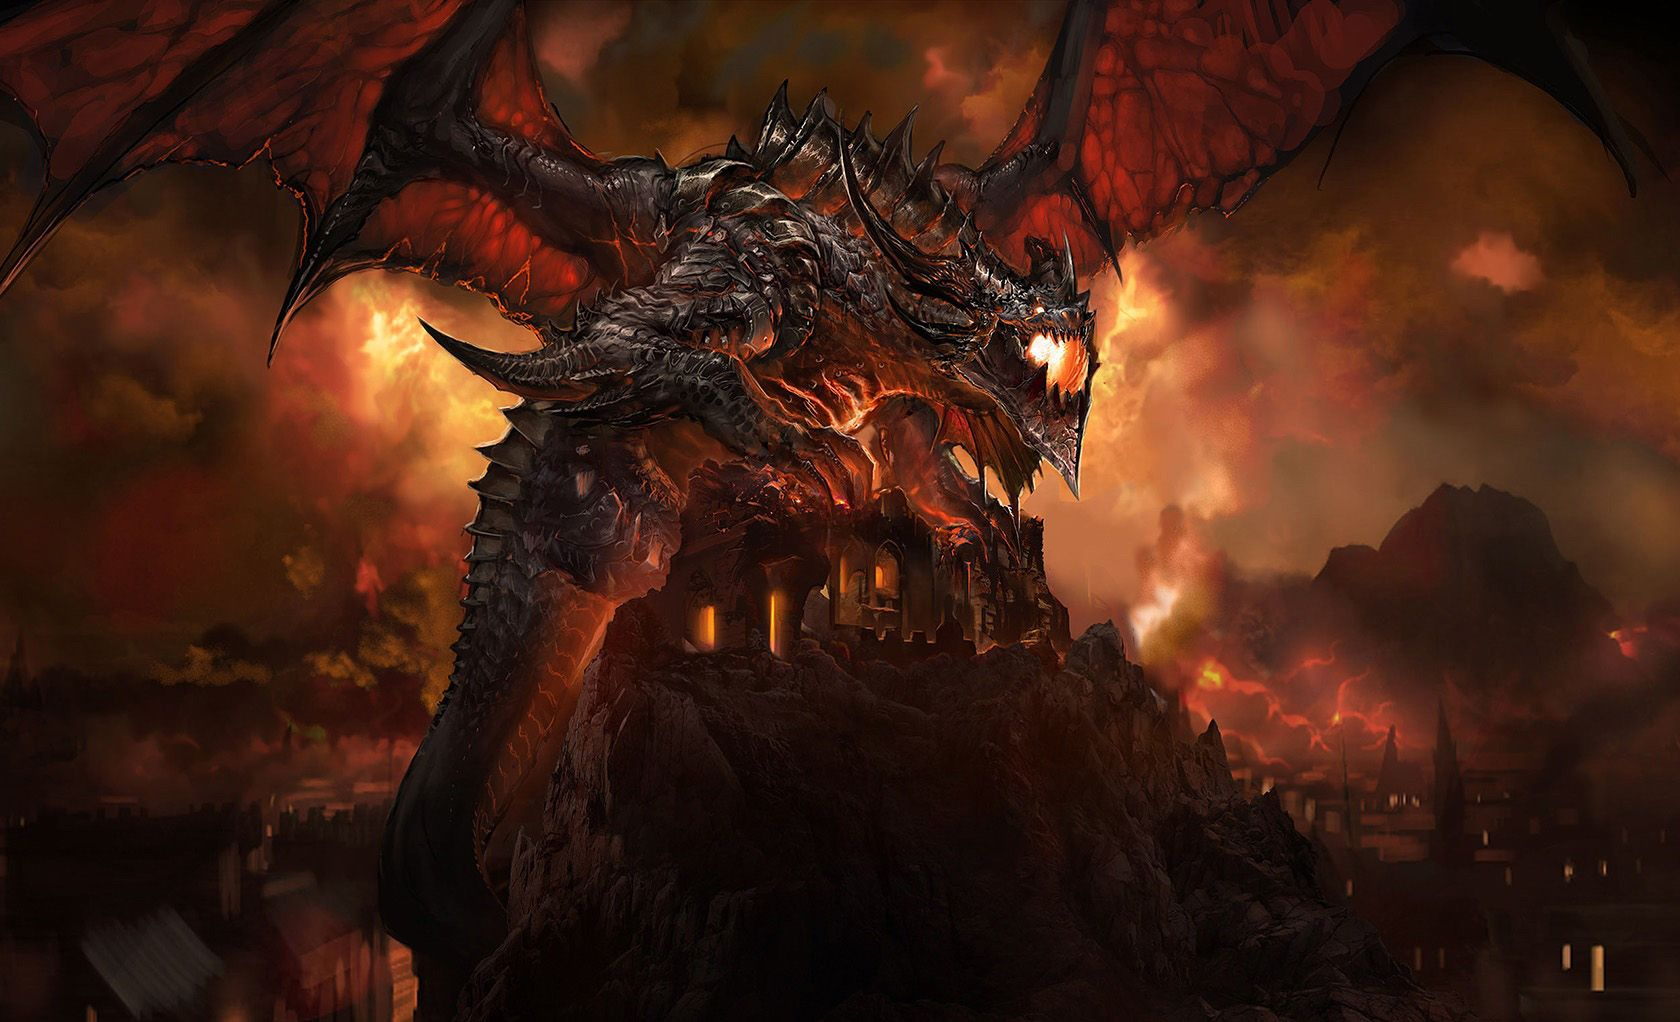
\includegraphics[width=0.7\linewidth]{img/WoW/deathwing.jpg}
	\end{center}

	Within the cavern of Infernalous contains one of three magical rings created by Myrddin, a red-gemmed ring. There are also other treasures that can be found within the cavern such as armor and shields from fallen foes who have traveled into the cavern. 

	\begin{center}
	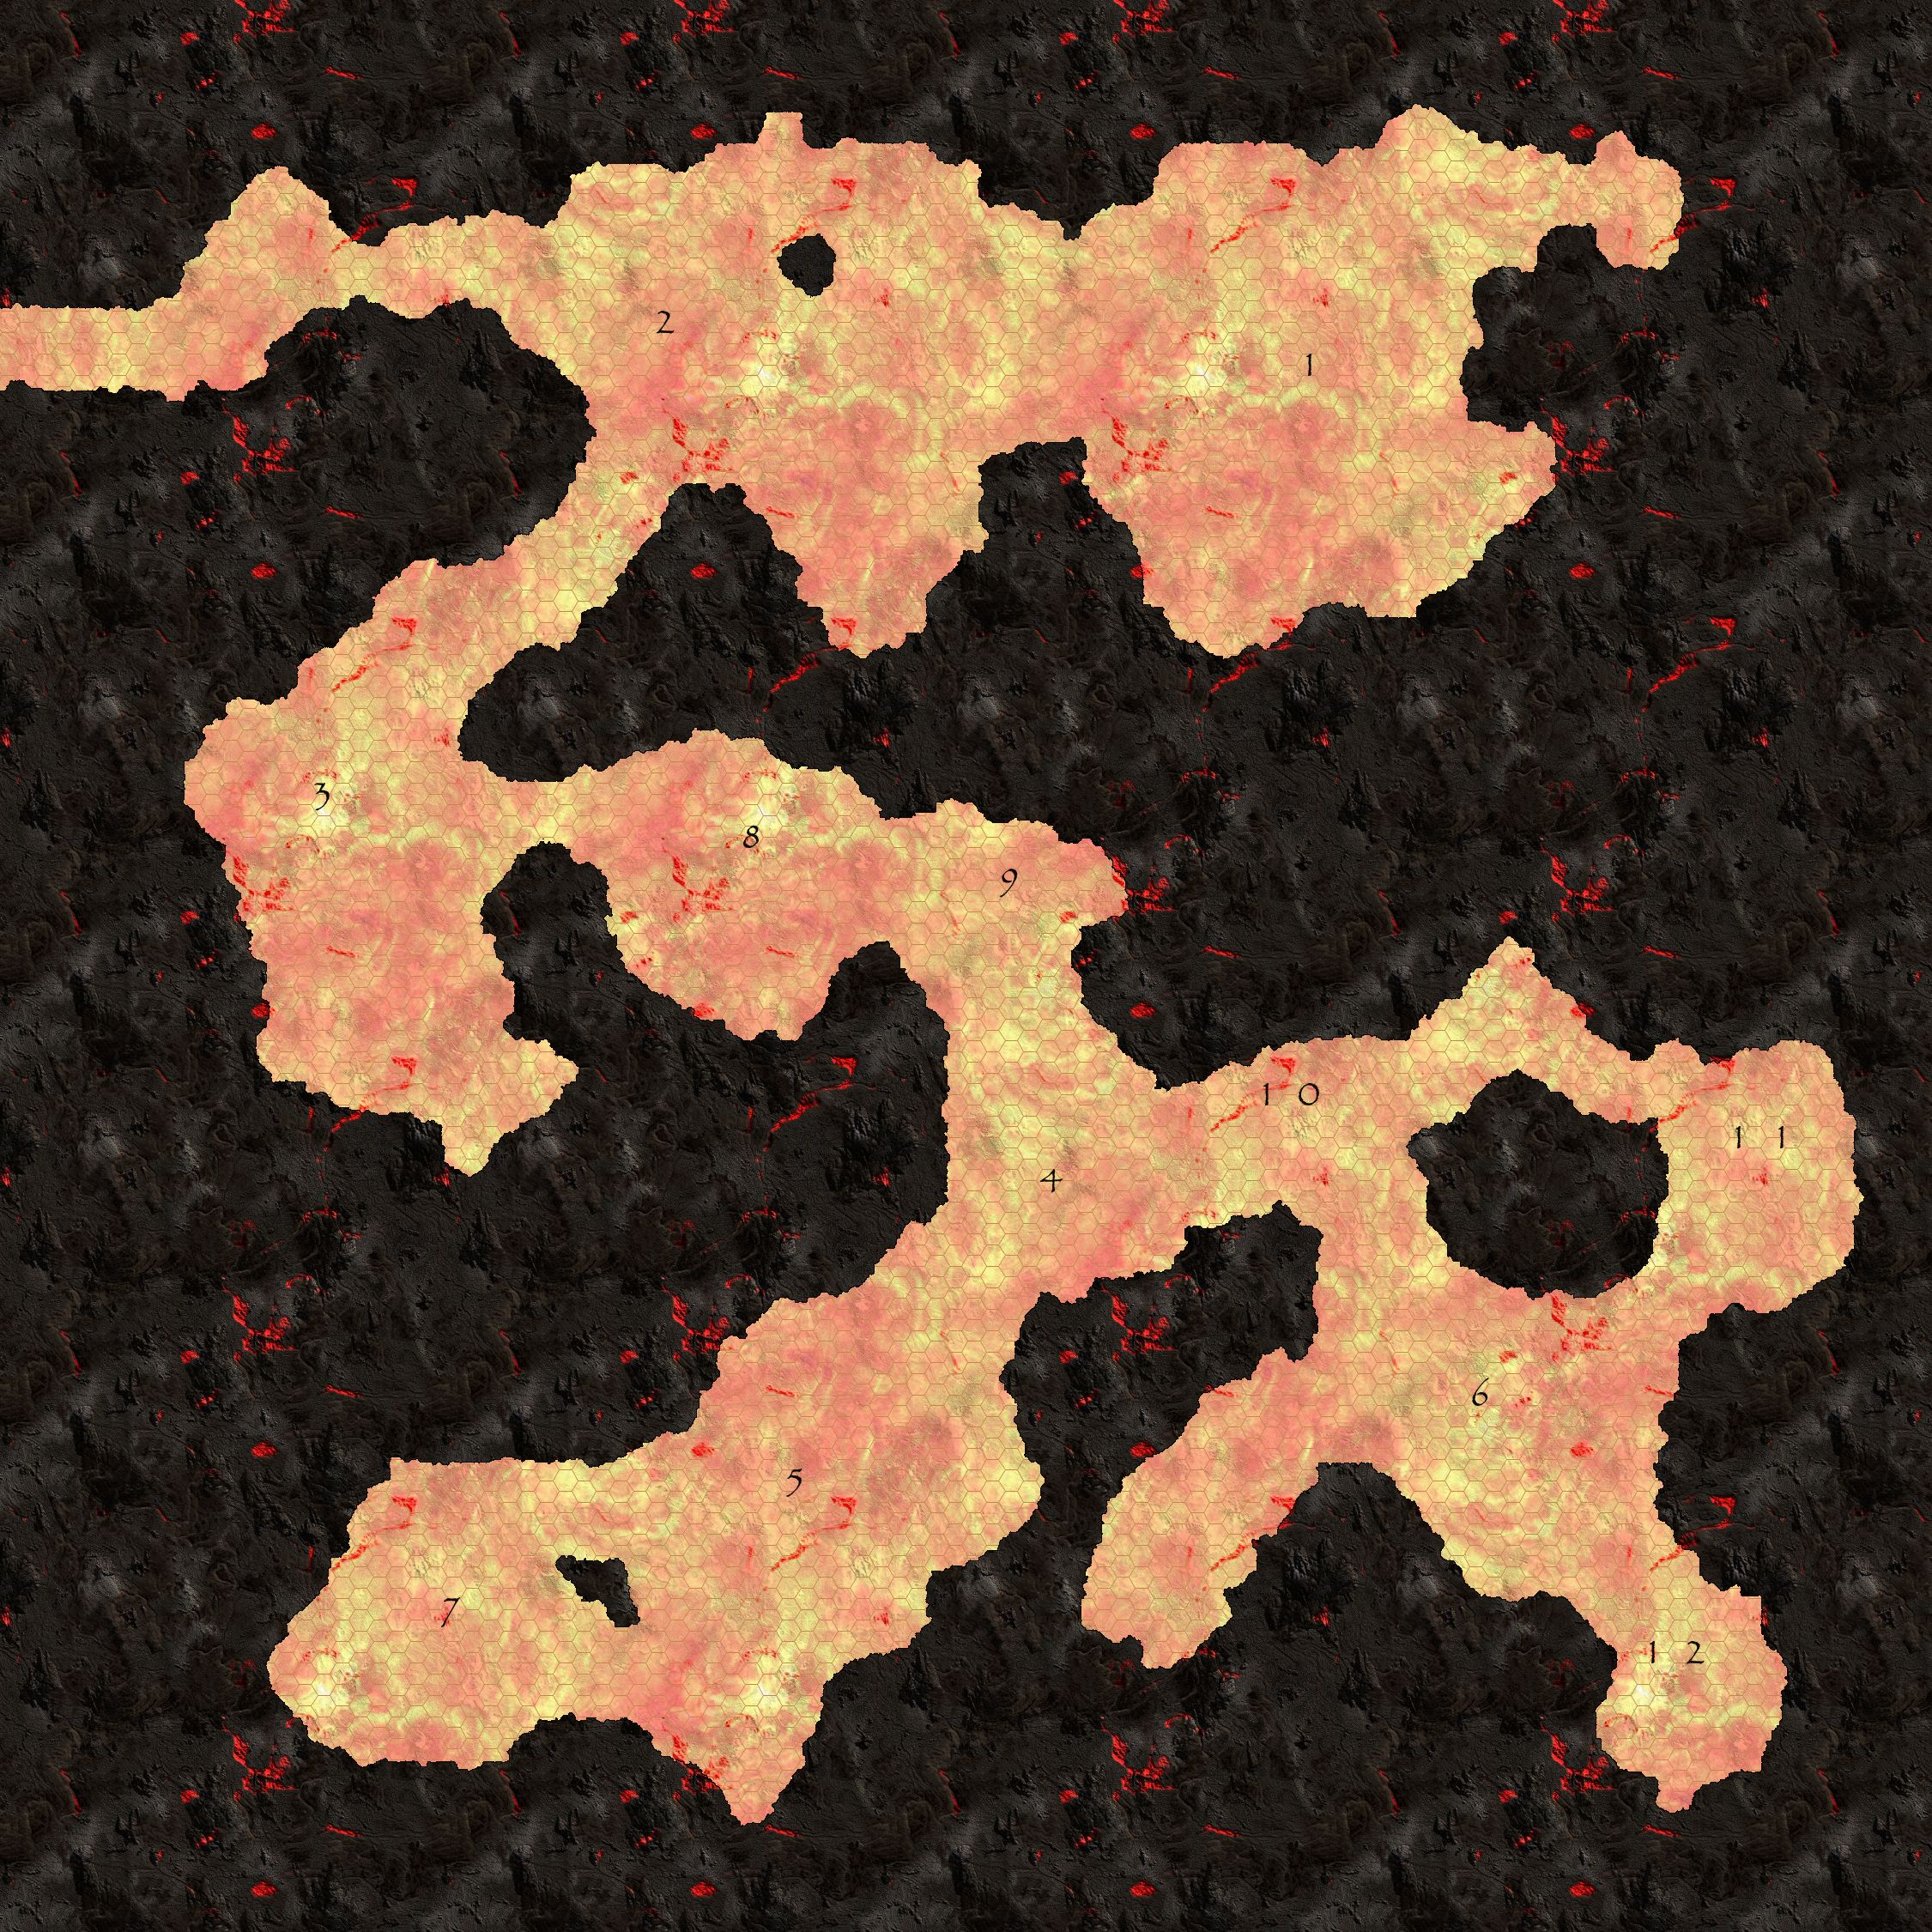
\includegraphics[width=0.7\linewidth]{img/maps/infernalous.jpg}
	\end{center}
\end{commentbox}

\begin{commentbox}{Aquaeleous}
	Aquaeleous is a large dragon created by Myrddin. The dragon is very old and extremely intelligent. This dragon is modeled after life and the lifeless and his abilities are in accordance with such. This dragon has poor hearing and sight, but can feel vibrations of the earth for those around. He can control minor aspects of matter by changing the materials around them and changing the states of matter.
	
	\begin{center}
	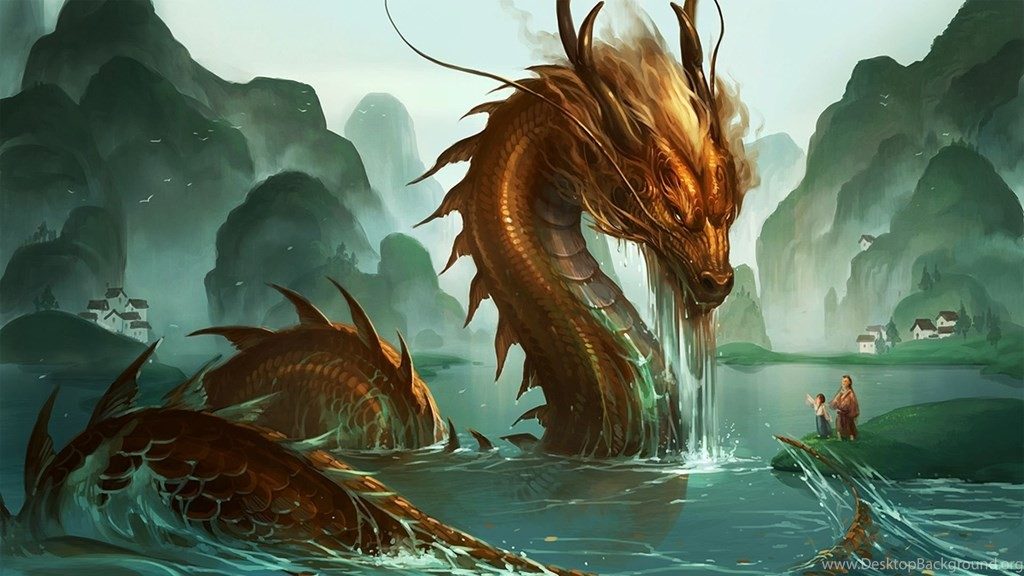
\includegraphics[width=0.7\linewidth]{img/waterdragon.jpg}
	\end{center}
	
	Within the cavern of Aquaeleous contains one of three magical rings created by Myrddin, a yellow-gemmed ring. There are also other treasures that can be found within the cavern such as staves, bows and other items from fallen foes who have traveled into the cavern. 
	
	\begin{center}
	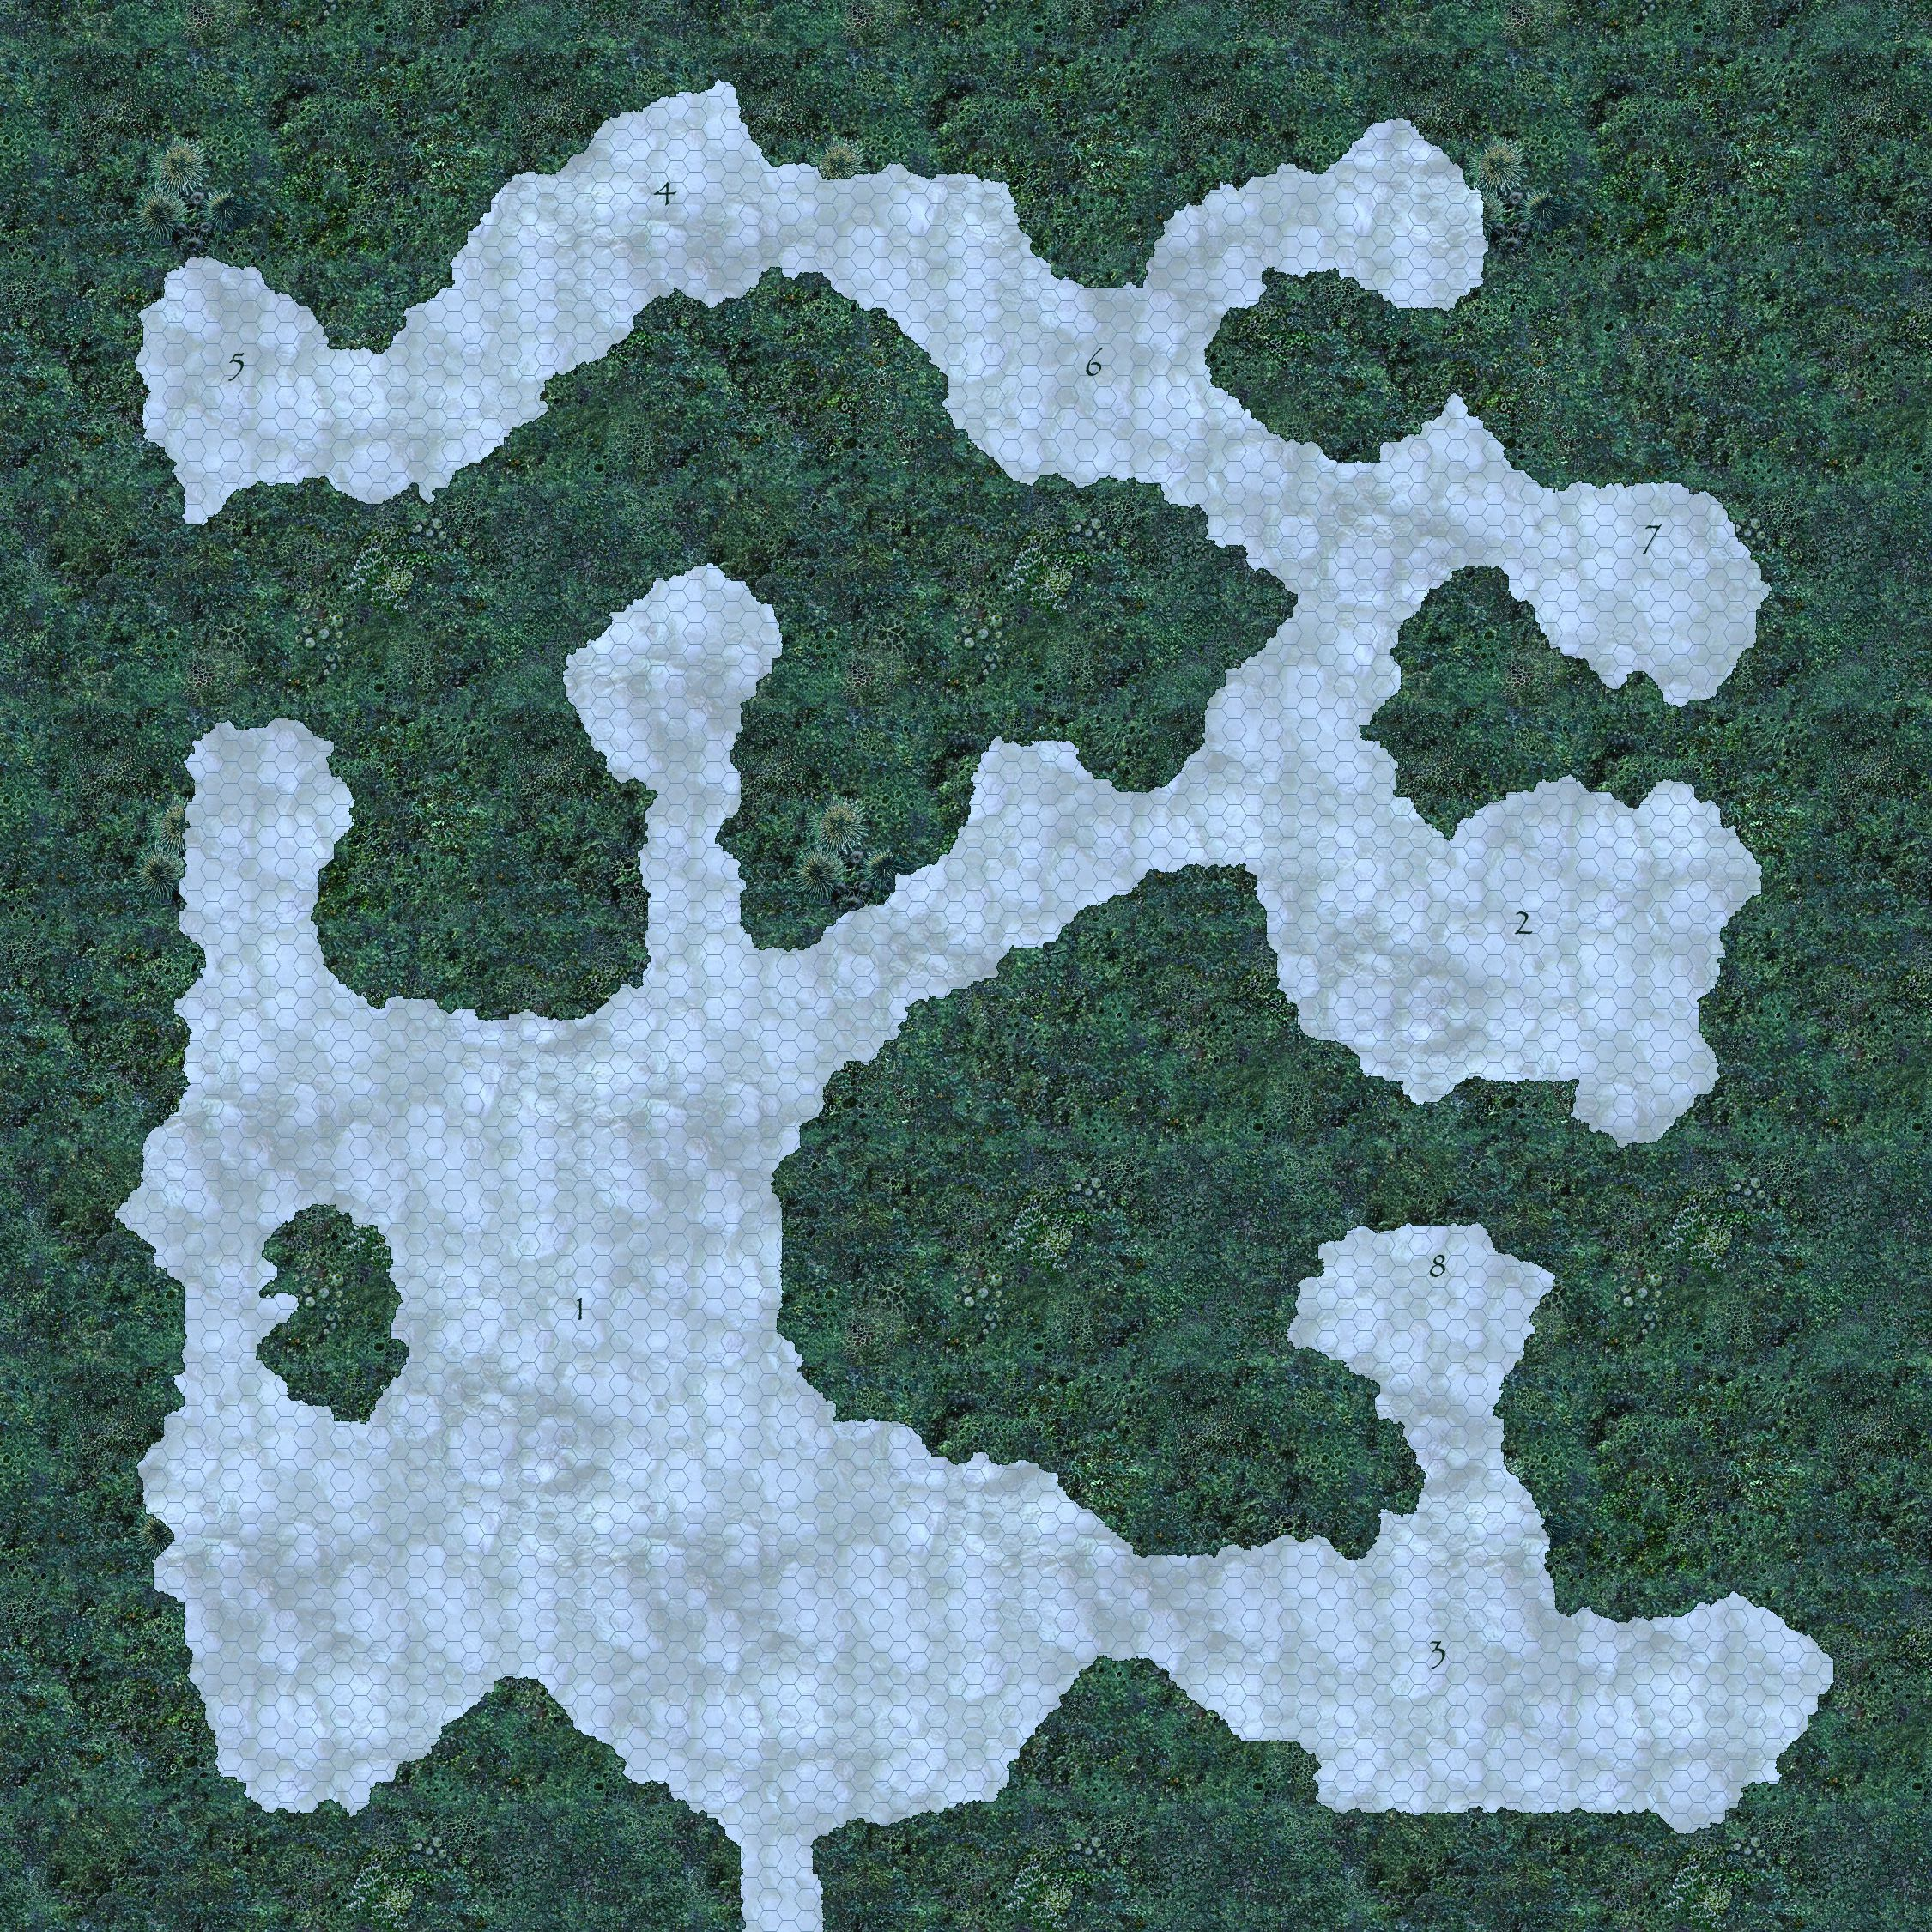
\includegraphics[width=0.7\linewidth]{img/maps/aquaeleous.jpg}
	\end{center}
\end{commentbox}


\begin{commentbox}{Crystalleous}
	Crystalleous is a large dragon created by Myrddin. The dragon is very old and extremely intelligent. This dragon is modeled after water and spirits and his abilities are in accordance with such. This dragon has poor hearing and sight, but can feel vibrations of the earth for those around. He can control minor aspects of time by changing the times of the atmospheric surroundings.
	
	\begin{center}
	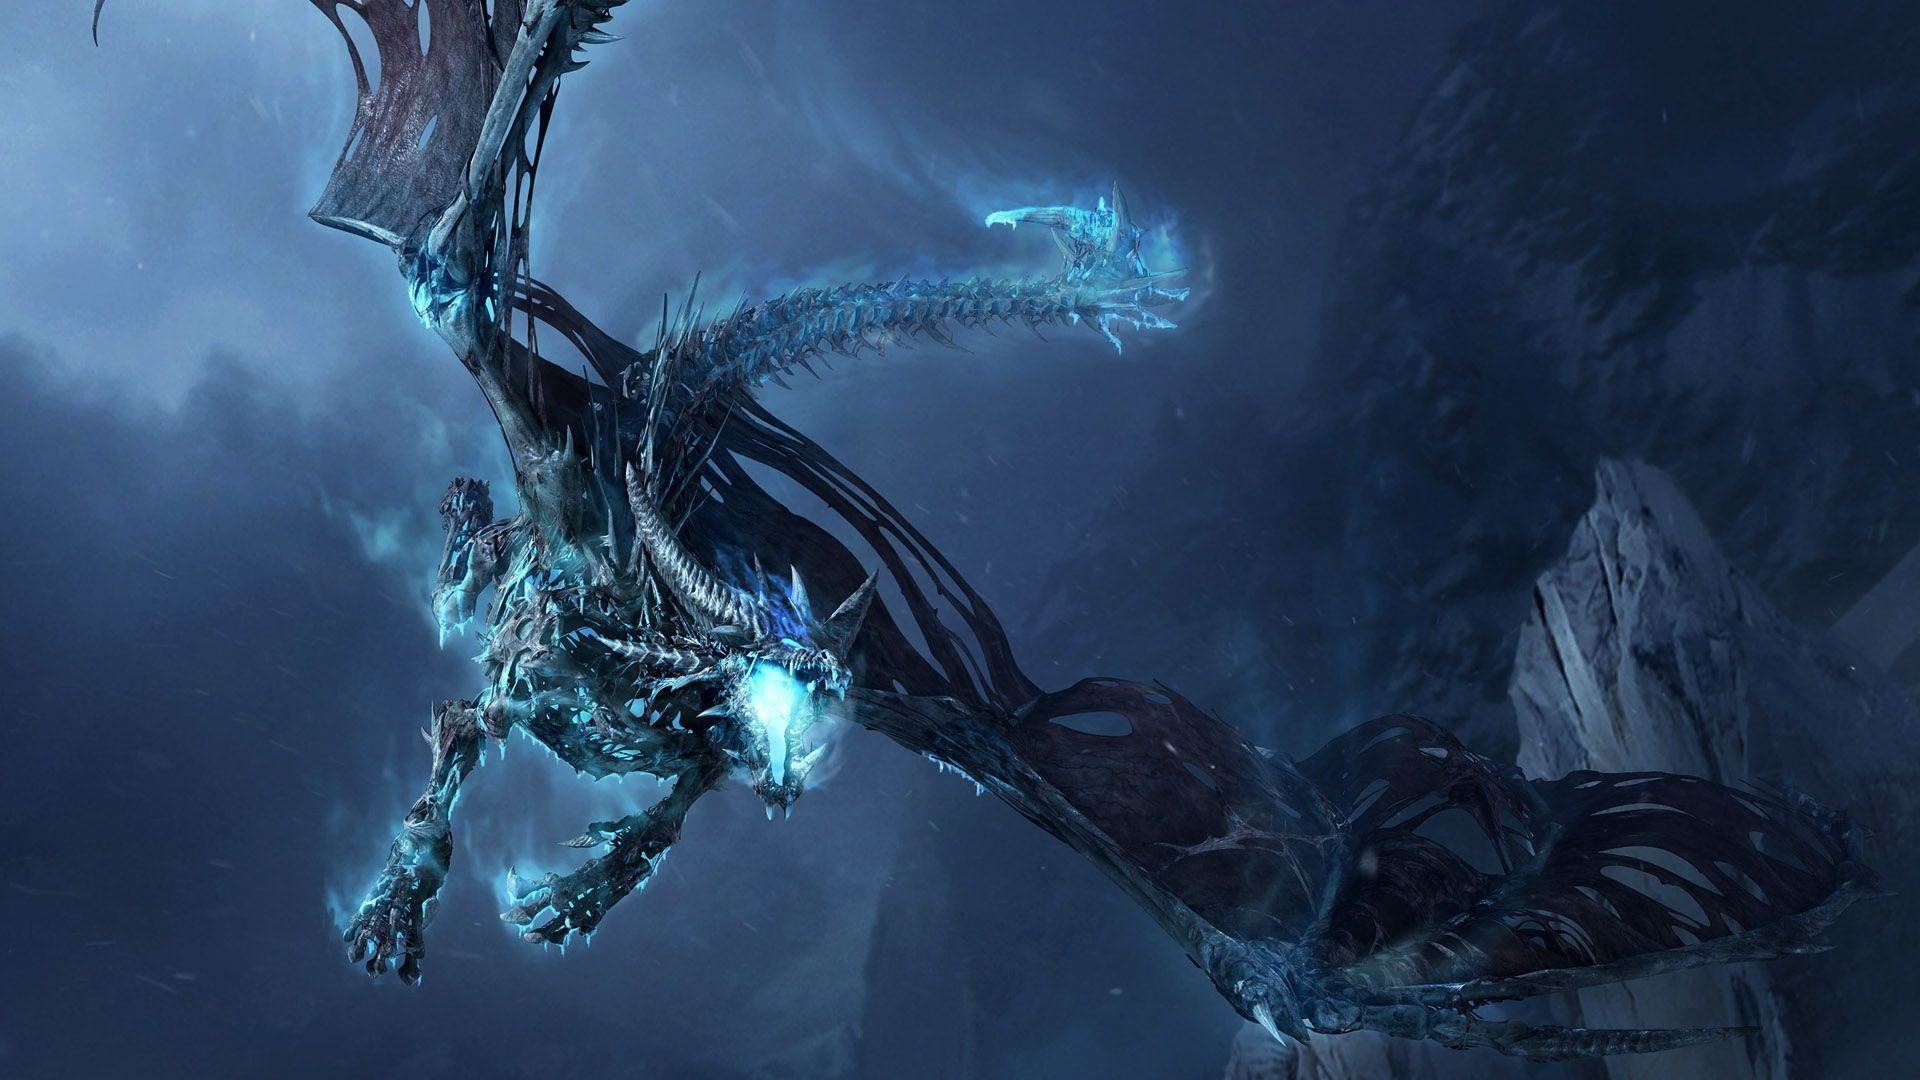
\includegraphics[width=0.7\linewidth]{img/WoW/crystaldragon.jpg}
	\end{center}

	Within the cavern of Crystalleous contains one of three magical rings created by Myrddin, a blue-gemmed ring. There are also other treasures that can be found within the cavern such as an ice rod, magic missile stave and other items from fallen foes who have traveled into the cavern. 
	
	\begin{center}
	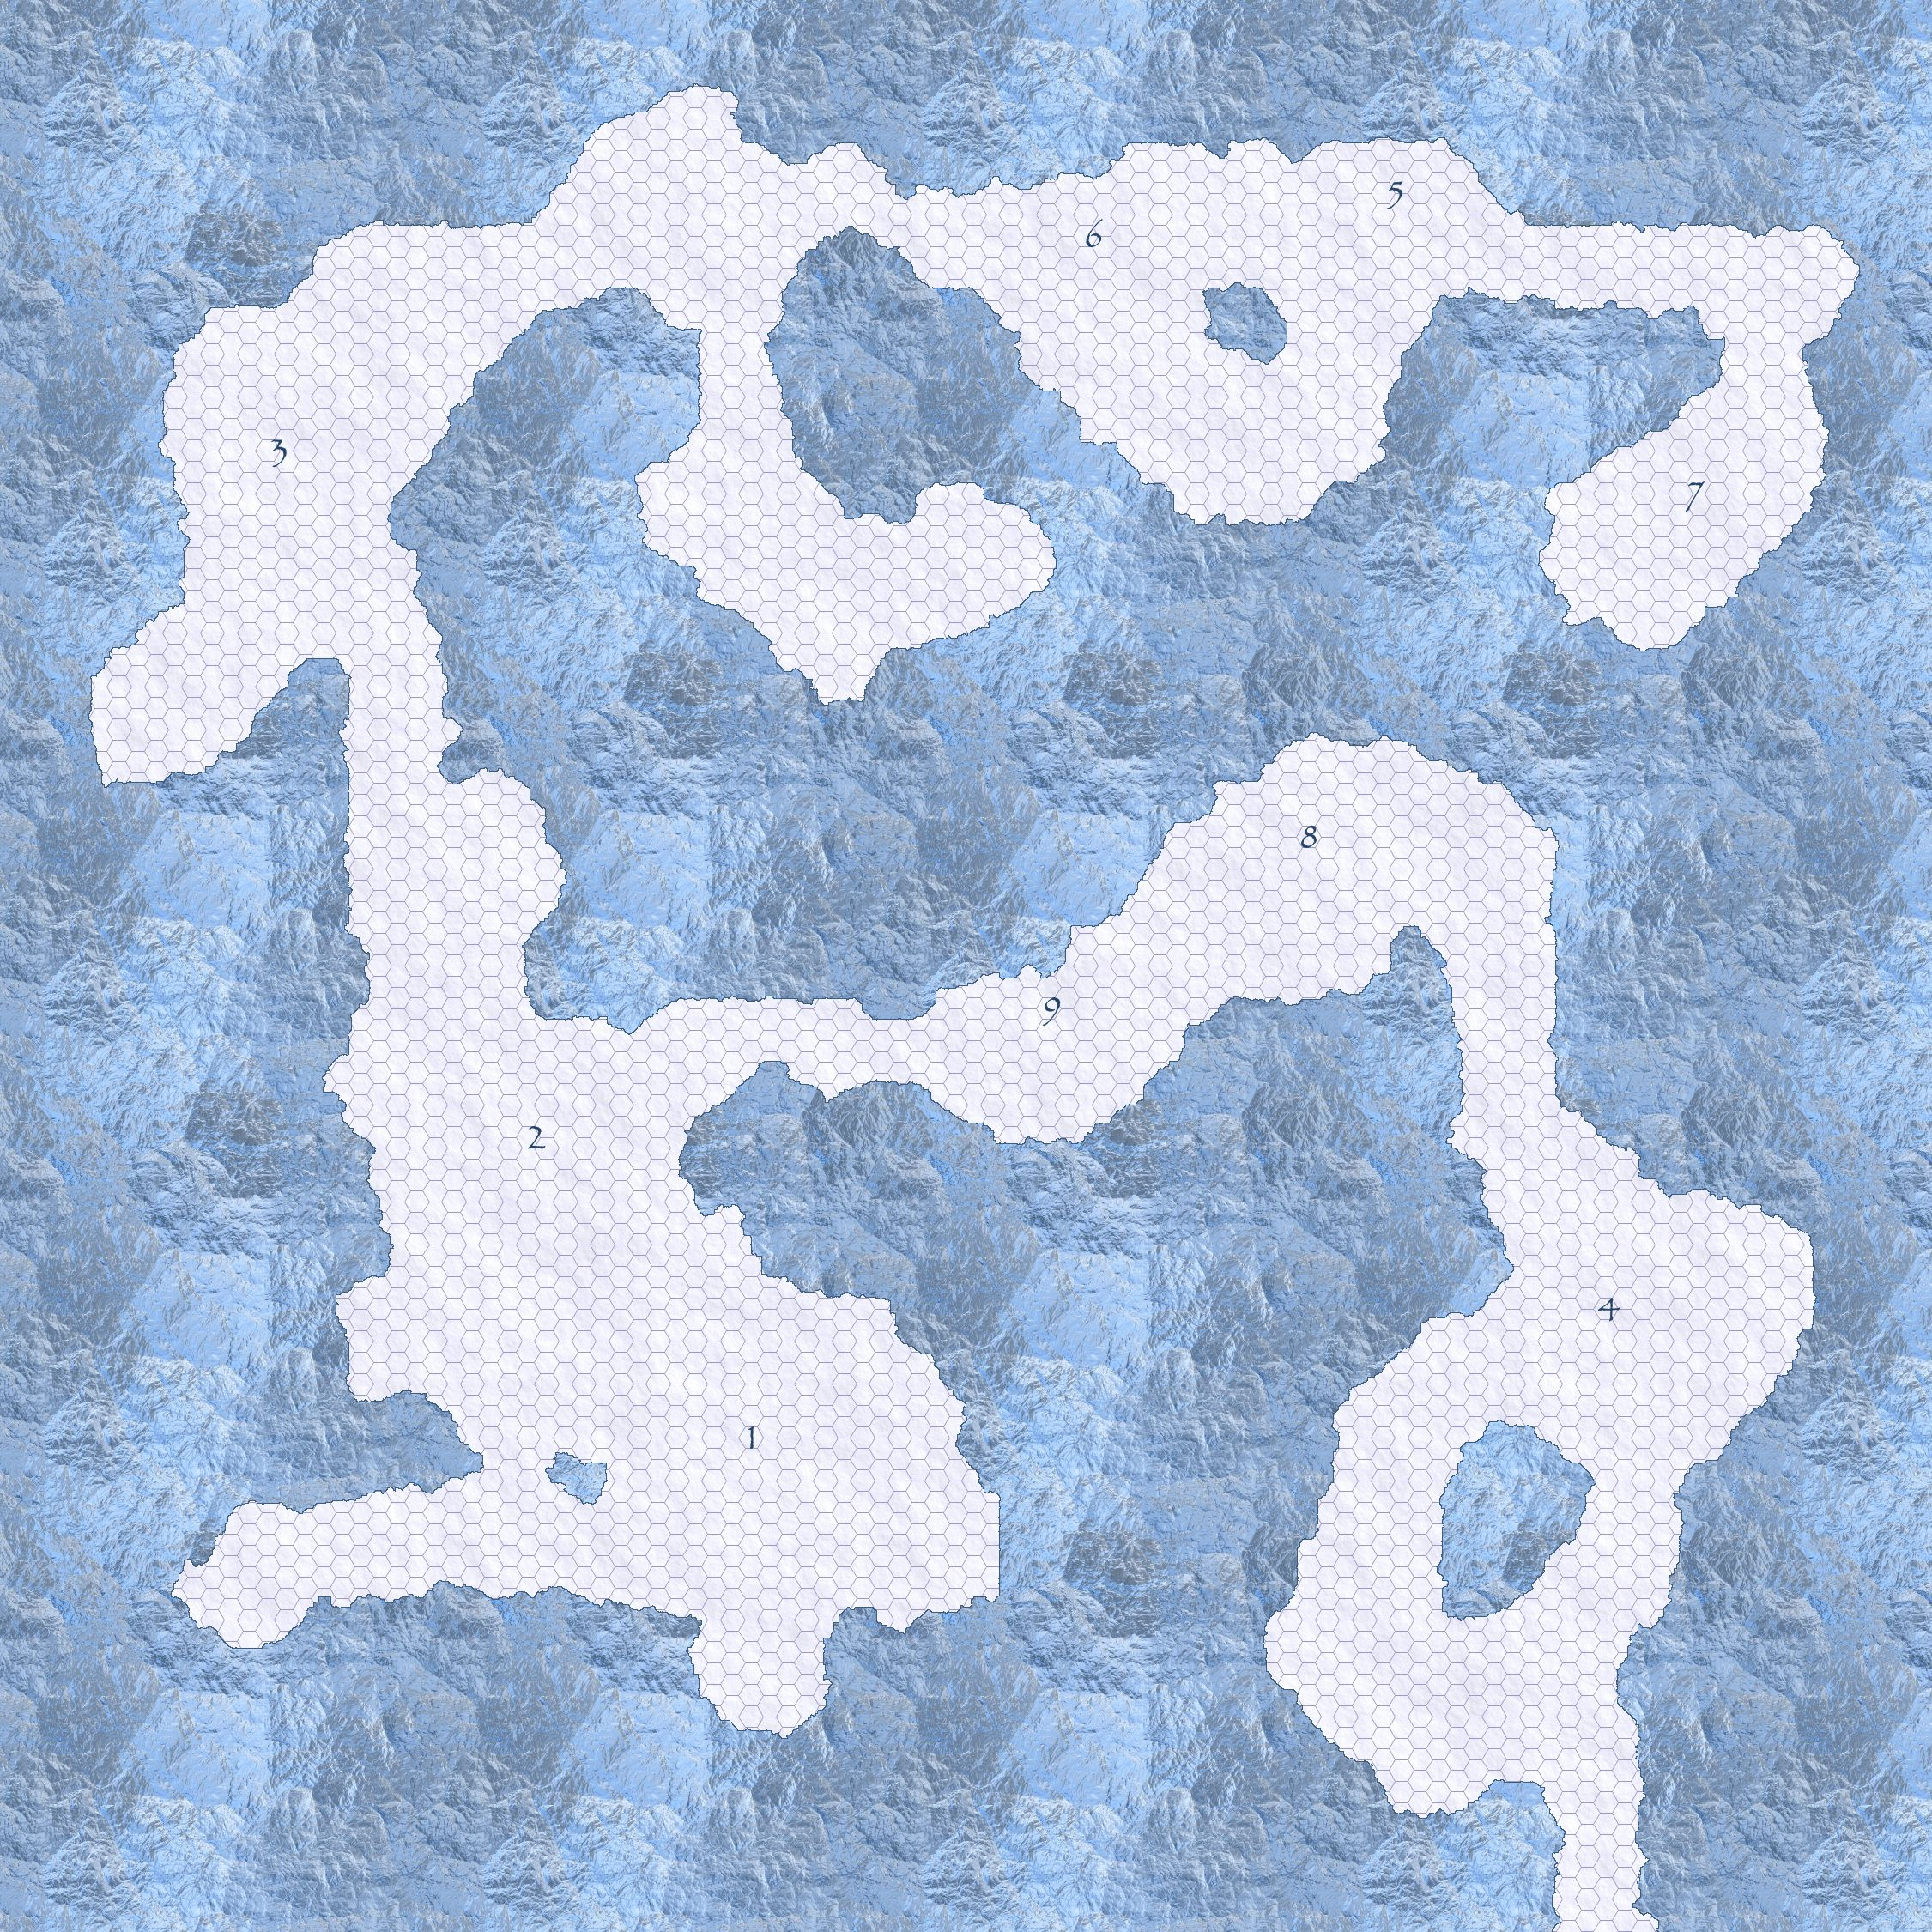
\includegraphics[width=0.7\linewidth]{img/maps/crystalleous.jpg}
	\end{center}
\end{commentbox}

\subsection{Xur'la}

Xur'la is a physical `god' created by Myrddin. Xur'la was created as a being to perform specific duties only a deity could perform. Xur'la was created to put a spiritual barrier around the Pluvian region and hide it from the sight of other ascended beings (gods). Xur'la is hidden deep in the Pluvian forest and can only be found if has the three rings of the trinity dragons are brought together.



